\documentclass[../documentation.tex]{subfiles}
 
\begin{document}
\section{Alkalmazáshoz szükséges műszaki feltételek elemzése}
\subsection{Projekt részletes leírása}
A projekt célja egy olyan robot demo hardveres és szoftveres kidolgozása, amely képes egy emberrel (továbbfejlesztés után akár egy másik robottal) lejátszani egy sakkjátszmát. A demo az ember-robot kollaboráció bemutatására szolgál, fontos szempont az interakció biztonságos megvalósítása mind az emberre, mind a környező tárgyakra tekintettel.\\

A megvalósításhoz a következő problémák megoldására van szükség:
\begin{enumerate}
	\item szükséges biztonsági funkciók beüzemelése,
	\item a bábuk helyzetének felismerése az egyes lépések előtt és után,
	\item a bábuk megfogása és mozgatása (ide tartozik a kalibráció és a referenciafelvétel),
	\item sakkalgoritmus beágyazása a programba,
	\item a sakkbábúk és a tábla megtervezése és megvalósítása,
	\item jelzés a robotkar számára, ha lépés történt.
\end{enumerate}
A felsorolt pontok a projekt során következőképpen kerültek kidolgozásra:
\begin{itemize}
	\item A bábuk helyzetének detektálása a projekt során QR-kód kereső és olvasó képfeldogozó eljárásokon alapul (a bábuk tetején található a kód). A kamera a roboton kerül rögzítésre.
	\item A bábuk mozgatása egy elektromosan vezérelt, párhuzamos megfogó (\angol{gripper}) segítségével történik.
	\item Ahhoz hogy a bábuk megfogása egyszerű legyen, azonos magasságú és azonos módszerrel megfogható bábuk készülnek.
	\item A biztonsági funkciók főként az tengelyekben ébredő plusz nyomatékok monitorozására és biztonsági zónák definiálására épül.
	\item A tábla és a robotkar, illetve a megfogó (egy jól definiált pontja) és a robotkar relatív helyzetének kalibrálására a robotvezérlő szoftverben elérhető alapfunkciók kerültek felhasználásra.
	\item A sakklépés megtörténtétét a robotvezérlőhöz kötött külső gombbal tudja a felhasználó jelezni.
	\item A képek fogadása, feldolgozása és a sakkalgoritmus futtatása mind a robotvezérlőn történik.
	\item Mivel a robotvezérlőn Java alapú környezet fut magas szinten, így a képfeldolgozó és a sakkozó programok is ebben lettek implementálva.
\end{itemize}

\subsection{A megfogó kialakításának és vezérlésének bemutatása}

\subsection{QR-kód generálás és képfeldolgozás}
A képfeldolgozáshoz lehetne saját mintát is használni a bábuk tetején, de a QR-kódok olvasására jól kidolgozott programok érhetőek el. A projekthez a nyílt forráskódú ZXing (``\angol{Zebra Crossing}'') program került felhasználásra\footnote{További információk és forráskód: https://github.com/zxing/zxing}. Ez a Java könyvtár (\angol{library}) alkamas különböző formátumú, egy- és kétdimenziós vonalkódokkal kapcsolatos képfeldolgozásra, ennek csak egyik eleme a QR-kód olvasás és generálás.

\subsubsection{A forráskód build-je}
A könyvtár egyszerű használatához célszerű .jar fájlokat generálni a forráskódból. Az első lépés a Github-on elérhető forráskód letöltése vagy klónozása a saját számítógépre. A programkód számos mappába és almappába van rendszerezve az egyes moduloknak megfelelően (pl.: core/ és javase/). \textbf{Fontos:} a mapparendszert olyan helyre tegyük a számítógépen, melynek elérési útjában nem található szóköz karakter (ékezetes karakter is probléma lehet)! Minden Java alapú modul esetén található egy pom.xml fájl, amit Apache Maven\footnote{Az Apache Maven program ingyenesen letölthető: https://maven.apache.org/} segítségével lehet használni.

Szükségünk van megfelelő java verzió telepítésére. A JRE (\angol{Java Runtime Environment}) helyett a JDK (\angol{Java Developement Kit}) valamelyik verzióját (a projekt jdk 10.0.2 verziót használ) érdemes telepíteni, ha fejlesztői funkciókat is igénybe szeretnénk venni (a JRE csomagot ez már tartalmazza). Az Apache Maven telepítése után szükségünk van az ehhez és a JDK-hoz tartozó környezeti változók beállítására. Ezt a Vezérlőpult->Rendszer->Speciális rendszerbeállítások->Környezeti változók...->Rendszerváltozók címszó alatt tehetjük meg. Szükségünk van egy `JAVA\_HOME' és egy `M2\_HOME' változóra (\ref{fig:envvar}. ábra).

Parancssorban navigáljunk a ZXing projekt gyökeréhez és futtassuk a `mvn install' parancsot a fordításhoz, a tesztekhez és az összes modul felépítéséhez. A ``-DskipTests'' paraméter hozzáadásával a unit teszteket kihagyhatjuk. Szükség lehet a `-Drat.ignoreErrors=true' paraméterre a licensz tesztekkel kapcsolatos problémák ignorálásához. A build folyamat akkor mondható sikeresnek, ha mindegyik modul felépítése sikeres (`ANDROID\_HOME' környezeti változó beállítása nélkül az Androidhoz kapcsolódó modulokat nem build-eli) (\ref{fig:buildsuccess}. ábra).

\begin{figure}[h]
\centering
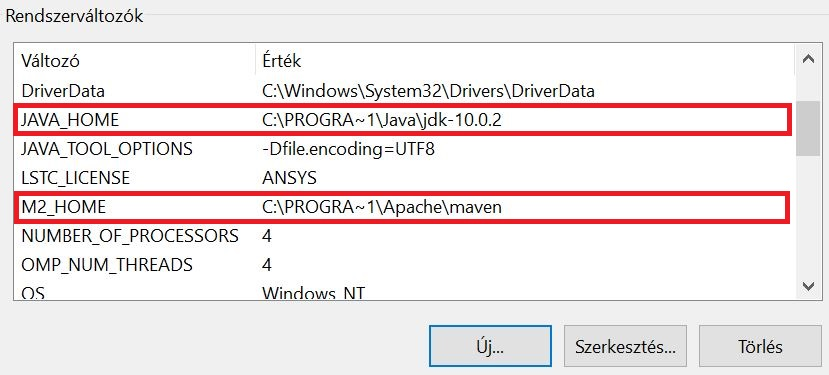
\includegraphics{env-variable}
\caption{Szükséges környezeti változók beállítása}
\label{fig:envvar}
\end{figure}

\begin{figure}[h]
\centering
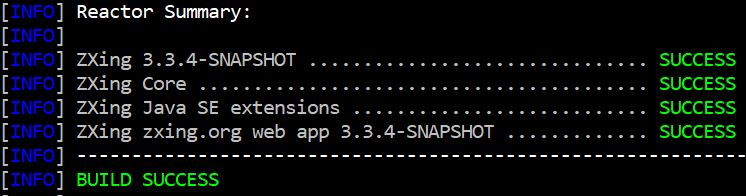
\includegraphics{zxingbuild}
\caption{Sikeres build végeredménye}
\label{fig:buildsuccess}
\end{figure}

A lefordított .jar fájlokat ezt követően az egyes modulokon belül találjuk. Például a lefordított \textit{core/} kód helye a \textit{core/target/core-x.y.z.jar}. Ezeket lehet beimportálni a képfeldolgozást megvalósító projektbe.

\subsubsection{ZXing könyvtár beimportálása és használata}
Az iiwa robotkart programozni Sunrise Workbench használatával a legegyszerűbb, ami egy JAVA Eclipse platformú szoftver. Emiatt praktikus okokból a szakdolgozat képfeldolgozási és sakkalgoritmus beágyazási része túlnyomó részt Eclipse-ben történt (verzió: 4.9.0)\footnote{Link: https://www.eclipse.org/}.

A könyvtár beimportálásához létrehoztam egy java projektet. Erre jobb egérgombbal kattintva elnavigáltam a `\angol{Configure Build Path...}' menüponthoz (\ref{fig:zxingimport}. ábra). A `\angol{Classpath}'-t kiválasztva jobb oldalt aktivizálódik az `\angol{Add External Jars...}' gomb. Kiválasztottam a \textit{core/} és a \textit{javase/} modulok .jar fájljait. Ezeken belül lehetőség van forráskód (\angol{Source attachment}) és dokumentáció (\angol{Javadoc location}) csatolására (\ref{fig:zxingimport}. ábra). `\angol{Apply and Close}' után megjelennek a csomagok a hivatkozott könyvtárak (\angol{Referenced libraries}) pont alatt.

\begin{figure}[h]
\centering
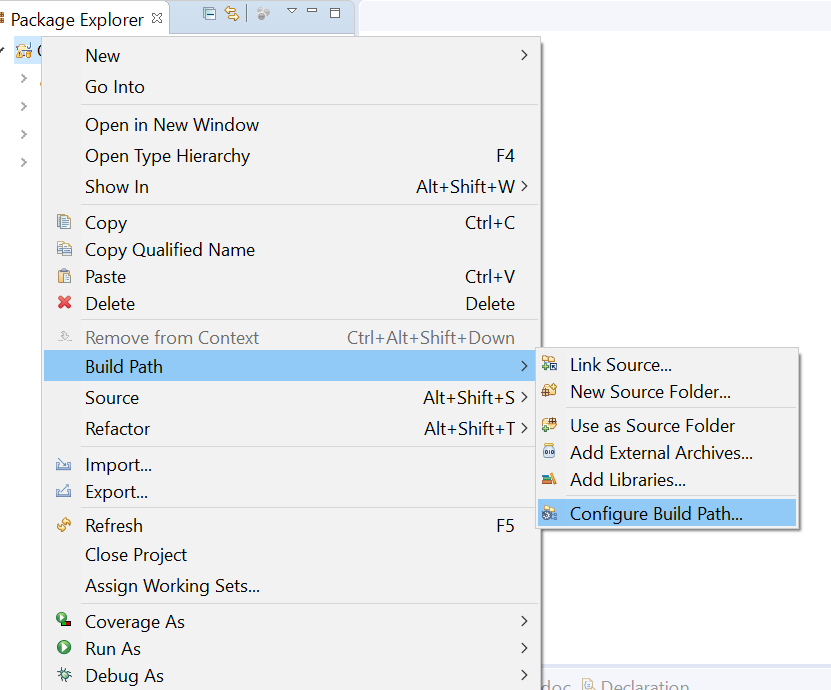
\includegraphics[scale=0.5]{buildpath}
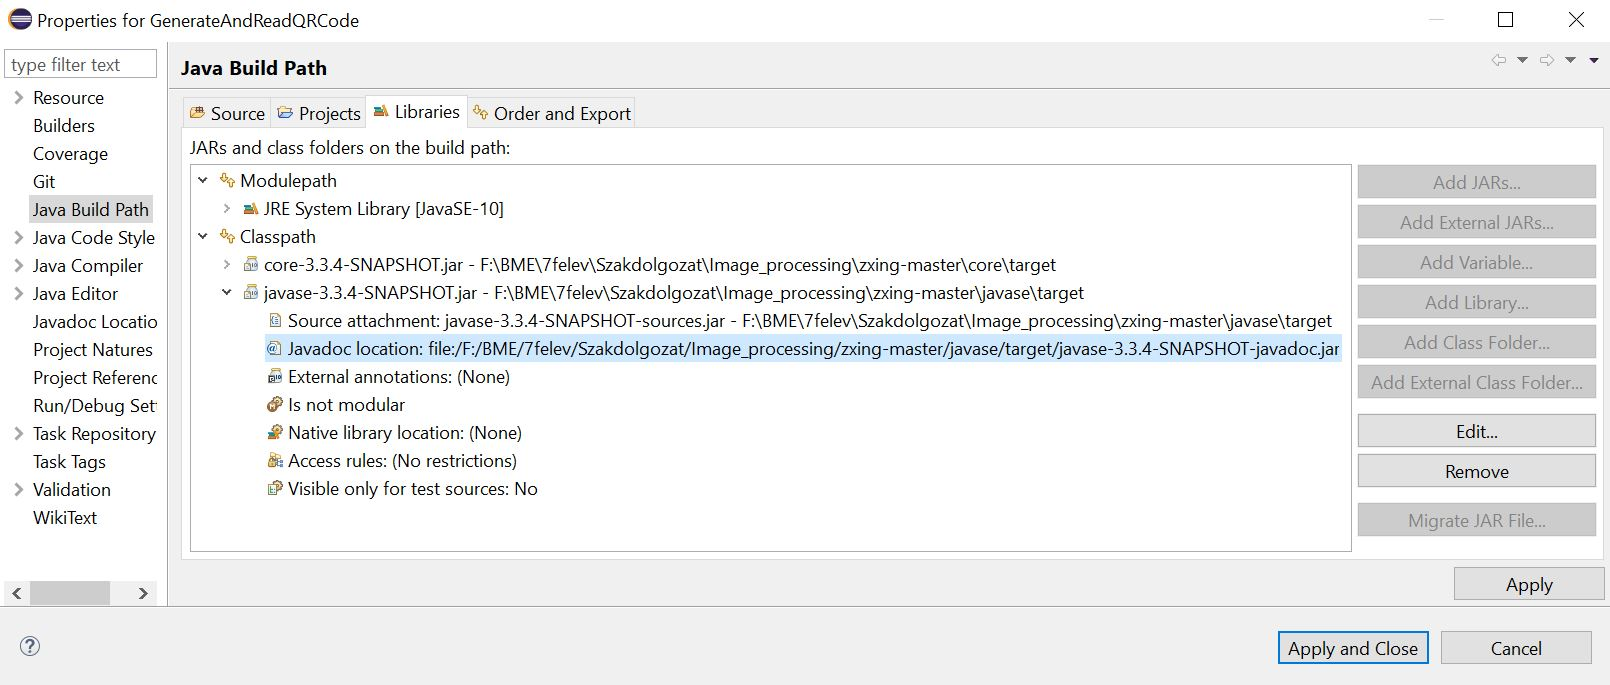
\includegraphics[scale=0.5]{zxingimport}
\caption{ZXing hozzáadása a hivatkozott könyvtárakhoz}
\label{fig:zxingimport}
\end{figure}












\end{document}